\section{Intervalos de confianza}
En la práctica, una muestra nunca es perfecta. Si elegimos un grupo de alumnos al azar, su
promedio va a variar respecto al promedio real de todo el colegio. Por eso, responder con un
solo número no alcanza para tomar decisiones institucionales seguras. La solución de la
estadística inferencial es la estimación por intervalos de confianza: en lugar de arriesgarnos
con un único resultado, calculamos un rango de valores (con un límite mínimo y uno máximo) que
tiene una alta probabilidad matemática de «atrapar» el verdadero promedio de la población.

La calidad de este rango depende de dos factores clave:
\begin{itemize}
  \item \textbf{El nivel de confianza ($1 - \alpha$):} nuestra certeza matemática (habitualmente
    90\% o 95\%). A mayor confianza, más ancho debe ser el intervalo para asegurar que no    dejamos el dato real afuera.
  \item \textbf{El tamaño de la muestra ($n$):} cuantos más alumnos evaluemos, menor es el    error estándar. Esto hace que la campana sea más angosta y la estimación sea muchísimo más
    exacta.
\end{itemize}

\AnalisisDescriptivo
Para poner a prueba la teoría retomamos el examen de química (\Variable{chemistry\_score}),
cuya media real es $\mu = 81{,}37$ y cuya desviación estándar es $\sigma = 5{,}26$. El perfil
completo de las notas es el siguiente:

\begin{TablaDatosFlexible}{L{0.26\linewidth} C{0.15\linewidth} L{0.46\linewidth}}{\textbf{Métrica estadística} & \textbf{Valor} & \textbf{Significado práctico}}

\TablaFilaFlexible{Total de datos ($N$) & 111 & Cantidad total de calificaciones registradas en el curso.}
\TablaFilaFlexible{Nota mínima & 75 & La calificación más baja obtenida en el examen de química.}
\TablaFilaFlexible{Nota máxima & 90 & La calificación más alta obtenida en el examen de química.}
\TablaFilaFlexible{Rango & 15 & La distancia total entre la nota más baja y la más alta.}
\TablaFilaFlexible{Media ($\mu$) & 81,37 & El promedio real de todo el curso (el centro de gravedad).}
\TablaFilaFlexible{Mediana & 80 & El valor central: el 50\% del curso sacó 80 o menos.}
\TablaFilaFlexible{Moda & 78 & La nota más común (se repite 34 veces en la lista).}
\TablaFilaFlexible{Desviación estándar ($\sigma$) & 5,26 & Qué tan dispersas están las notas individuales frente al promedio.}
\TablaFilaFlexible{Varianza ($\sigma^2$) & 27,62 & Medida matemática de la dispersión de los datos.}

\end{TablaDatosFlexible}

\subsection{Puesta a prueba de la teoría}
La simulación selecciona grupos de alumnos al azar con tres tamaños diferentes ($n = 10$,
$n = 20$ y $n = 30$) y a cada grupo le calcula su intervalo de confianza al 95\%. El cálculo
combina los dos factores clave vistos al principio:
\begin{equation*}
  IC = \bar{x} \pm E, \qquad
  E = Z_{\alpha/2} \cdot \sigma_{\bar{x}}, \qquad
  \sigma_{\bar{x}} = \frac{\sigma}{\sqrt{n}}
\end{equation*}
\PalabraClave{Cómo se toman los datos:} Con un nivel de confianza del 95\% el valor crítico es
$Z_{\alpha/2} = 1{,}96$. El error estándar de la media cae al agrandar el grupo y, como el
margen de error $E$ es proporcional a ese error estándar, el intervalo se achica solo por el
hecho de evaluar a más alumnos. Como en la simulación conocemos la media real de la población,
construimos los intervalos centrados en $\mu = 81{,}37$ para verificar si el modelo atrapa el
valor verdadero.

\TituloGrafico{Cobertura de los intervalos de confianza}

\begin{figure}[H]
    \centering
    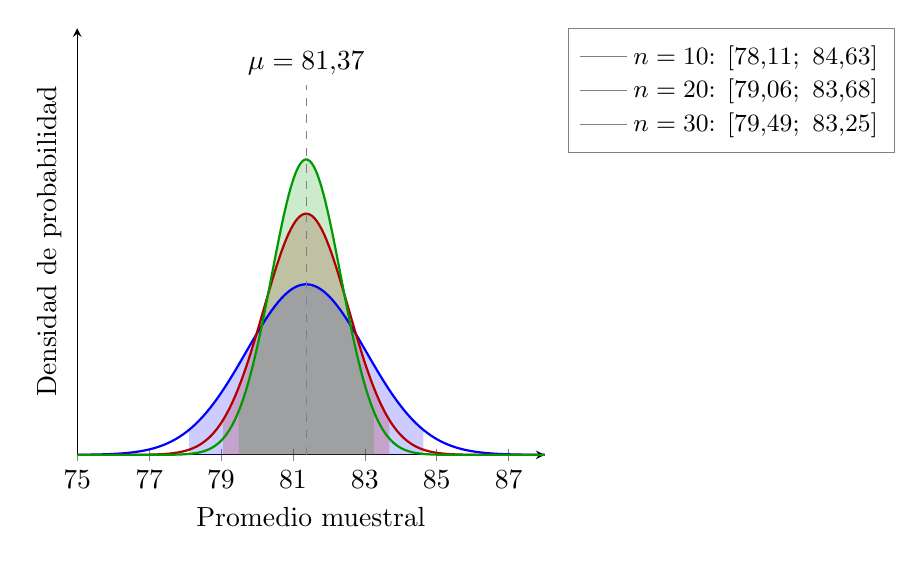
\begin{tikzpicture}
        % Función de densidad normal con parámetros configurables.
        \pgfmathdeclarefunction{dens}{3}{%
          \pgfmathparse{1/(#3*sqrt(2*pi))*exp(-((#1-#2)^2)/(2*(#3)^2))}%
        }
        \begin{axis}[
            width=0.62\textwidth,
            height=7cm,
            xlabel={Promedio muestral},
            ylabel={Densidad de probabilidad},
            xmin=75, xmax=88,
            ymin=0, ymax=0.6,
            xtick={75,77,79,81,83,85,87},
            ytick=\empty,
            axis lines=left,
            samples=200,
            legend style={at={(1.05,1.0)}, anchor=north west, font=\small,
                fill=white, draw=black!50, fill opacity=1, text opacity=1,
                inner sep=4pt, cells={anchor=west}},
            legend cell align=left,
            clip=false,
        ]
            % Áreas sombreadas: cada intervalo de confianza bajo su propia campana.
            \addplot[fill=blue, draw=none, fill opacity=0.20, domain=78.11:84.63]
                {dens(x,81.37,1.6634)} \closedcycle;
            \addplot[fill=red!70!black, draw=none, fill opacity=0.20, domain=79.06:83.68]
                {dens(x,81.37,1.1762)} \closedcycle;
            \addplot[fill=green!60!black, draw=none, fill opacity=0.20, domain=79.49:83.25]
                {dens(x,81.37,0.9603)} \closedcycle;
            % Campanas de los promedios muestrales.
            \addplot[blue, thick, domain=75:88] {dens(x,81.37,1.6634)};
            \addlegendentry{$n = 10$: $[78{,}11;\ 84{,}63]$}
            \addplot[red!70!black, thick, domain=75:88] {dens(x,81.37,1.1762)};
            \addlegendentry{$n = 20$: $[79{,}06;\ 83{,}68]$}
            \addplot[green!60!black, thick, domain=75:88] {dens(x,81.37,0.9603)};
            \addlegendentry{$n = 30$: $[79{,}49;\ 83{,}25]$}
            % Media real de la población.
            \draw[dashed, gray] (axis cs:81.37,0) -- (axis cs:81.37,0.52)
                node[above, black] {$\mu = 81{,}37$};
        \end{axis}
    \end{tikzpicture}
    \caption{Distribución teórica de los promedios muestrales con el área sombreada que
    representa cada intervalo de confianza al 95\%. Todos los intervalos están centrados en la
    media real $\mu = 81{,}37$ y se estrechan a medida que crece el tamaño del grupo.}
    \label{fig:intervalos_campanas}
\end{figure}

\PalabraClave{Lo que revelan las curvas de la simulación:}
\begin{itemize}
  \item \textbf{Muestra pequeña ($n = 10$) | Curva azul (baja y ancha):} Los promedios
    individuales saltan de forma muy inestable (varían entre 80,40 y 83,30 puntos). El
    intervalo queda muy abierto y genera un margen de error grande de $\pm\,3{,}26$ puntos.
    Precisión muy baja: los grupos chicos no logran compensar las notas extremas.
  \item \textbf{Tamaño medio ($n = 20$) | Curva roja (intermedia):} Al promediar más alumnos,
    los extremos se empiezan a compensar y el rango de los promedios se achica (79,40 a
    83,85). La campana se vuelve un poco más alta y angosta, y el margen de error baja a
    $\pm\,2{,}31$ puntos. Precisión aceptable.
  \item \textbf{Tamaño óptimo ($n = 30$) | Curva verde (alta y angosta):} Los promedios se
    compactan fuertemente en el centro (79,63 a 83,00), amontonándose en el valor real. La
    campana es la más puntiaguda de la simulación y consigue el menor margen de error: apenas
    $\pm\,1{,}88$ puntos. Precisión óptima, alcanzando la convergencia que dicta el Teorema
    Central del Límite.
\end{itemize}

\subsection{Cuadro comparativo}
El cálculo completo de los tres intervalos, lado a lado:

\begin{TablaDatosFlexible}{L{0.31\linewidth} C{0.16\linewidth} C{0.16\linewidth} C{0.16\linewidth}}{\textbf{Parámetro} & \textbf{$n = 10$} & \textbf{$n = 20$} & \textbf{$n = 30$}}

\TablaFilaFlexible{Nivel de confianza ($1 - \alpha$) & \multicolumn{3}{c}{95\%}}
\TablaFilaFlexible{Valor crítico ($Z_{\alpha/2}$) & \multicolumn{3}{c}{$1{,}96$}}
\TablaFilaFlexible{Error estándar ($\sigma_{\bar{x}} = \frac{\sigma}{\sqrt{n}}$) & 1,66 & 1,18 & 0,96}
\TablaFilaFlexible{Margen de error ($E = Z_{\alpha/2} \cdot \sigma_{\bar{x}}$) & $\pm\,3{,}26$ & $\pm\,2{,}31$ & $\pm\,1{,}88$}
\TablaFilaFlexible{Límite inferior ($\mu - E$) & 78,11 & 79,06 & 79,49}
\TablaFilaFlexible{Límite superior ($\mu + E$) & 84,63 & 83,68 & 83,25}
\TablaFilaFlexible{Rango de medias muestrales & 80,40 – 83,30 & 79,40 – 83,85 & 79,63 – 83,00}
\TablaFilaFlexible{Promedio global obtenido & 81,39 & 81,56 & 81,24}
\TablaFilaFlexible{\footnotesize Lectura & \footnotesize Dispersión alta & \footnotesize Estable & \footnotesize Precisión óptima}

\end{TablaDatosFlexible}

\Interpretacion
El gráfico comparativo de campanas demuestra visualmente la regla de oro: a mayor tamaño de
muestra ($n$), el intervalo de confianza se vuelve más angosto. Esto significa que logramos una
mejor estimación de la verdadera media poblacional reduciendo el error al mínimo. Además, los
tres intervalos contienen la media real ($\mu = 81{,}37$) y los tres promedios globales
obtenidos (81,39; 81,56 y 81,24) caen dentro de sus propios intervalos, confirmando que la
media muestral es el mejor estimador posible para conocer la realidad de los alumnos.